\section{Historical Experiments}
\label{app:historical_synthetic}

\subsection{Experimental setup}
\label{sec:exp_setup}

\textbf{Environment.}  A 1-D continuous navigation task with position $p\in[-10,10]$ and velocity action $a\in[-1,1]$.  The reward vector is 2-dimensional, $\mathbf{r}=(r_{\text{safety}}, r_{\text{progress}})$, constructed so that \emph{each mode collapses one objective to a different state feature}: in ``safety'' mode $r_{\text{safety}}$ is position-responsive while $r_{\text{progress}}$ collapses to the action; in ``progress'' mode the roles reverse; in ``balanced'' mode both are position-responsive.  This creates different mode-specific return geometries; all simplex preferences remain valid scalarized utilities.  Three modes cycle deterministically every \texttt{switch\_interval}$=300$ steps with ground-truth anchors $w_0{=}[0.85,0.15]$ (safety-dominated), $w_1{=}[0.15,0.85]$ (progress-dominated), $w_2{=}[0.5,0.5]$ (balanced).

\textbf{Algorithms.}  We compare five methods, all sharing the same actor--critic backbone and weight-conditioned policy $\pi(a\mid s, w)$; they differ \emph{only} in how preference weights are sampled and whether the cone estimator is active:
\begin{itemize}[topsep=1pt,leftmargin=1.3em]
    \item \textbf{BAMOR-TC}: Target Cone with frozen-uniform belief. Cone statistics $\hat w_{\mathrm{anchor}}$ are estimated from reward variance; $w \sim \mathrm{Dir}(\kappa \cdot \tilde w)$ with $\kappa{=}20$. No online mode-change detector.
    \item \textbf{BAMOR $+$ surprise}: BAMOR-TC with the Mahalanobis online change-point detector active (threshold$=7$, cooldown$=290$ steps, warm-up$=150$).
    \item \textbf{BAMOR $-$ Cone}: historical ablation retaining the surprise detector while disabling the cone. The current implementation uses $\mathrm{Dir}(\mathbf 1)$; the historical output files do not record the sampler concentration.
    \item \textbf{Uniform-sampling}: $w \sim \mathrm{Dir}(\mathbf{1})$ every step, no cone, no belief---a preference-conditioned actor--critic baseline.
    \item \textbf{Fixed-weight}: $w=[0.5,0.5]$ throughout training, no cone, no belief---a scalar sanity baseline.
\end{itemize}
All methods train for $100{,}000$ environment steps with identical network sizes, learning rates, replay buffers, and a 20-seed sweep on a shared GPU cluster.  Final performance is measured by hypervolume (HV) against reference point $(-5,-5)$, evaluated (i) globally over a dense grid of $21$ preference weights under the mode-switching schedule and (ii) per mode by locking the environment to a fixed mode and re-evaluating on $11$ weights.

% ── 6.2 Main result ─────────────────────────────────────────────────────────
\subsection{Historical synthetic results}

\begin{table}[t]
\centering\small
\caption{Hypervolume (HV) on the synthetic non-stationary MO environment at 100K steps (5 seeds).  Mode anchors are $w_0{=}[0.85,0.15]$, $w_1{=}[0.15,0.85]$, $w_2{=}[0.5,0.5]$.  Reference point $(-5,-5)$.  Bold = best per column; BAMOR dominates Mode~1 (skewed cone, $+28.2\%$ over Uniform) and wins on three of four columns.}
\label{tab:main_results}
\begin{tabular}{lcccc}
\toprule
Method & HV overall & HV Mode 0 & HV Mode 1 & HV Mode 2 \\
\midrule
BAMOR (full) & $130.9{\pm}16.9$ & \textbf{$21.9{\pm}0.4$} & \textbf{$48.2{\pm}2.4$} & \textbf{$125.5{\pm}27.7$} \\
BAMOR$-$Cone & \textbf{$136.0{\pm}17.1$} & $19.8{\pm}2.7$ & $42.7{\pm}6.5$ & $124.7{\pm}24.9$ \\
BAMOR$-$Surprise & $115.2{\pm}39.6$ & $21.6{\pm}0.6$ & $36.0{\pm}8.3$ & $109.5{\pm}45.0$ \\
Uniform-sampling & $122.3{\pm}54.8$ & $21.1{\pm}1.3$ & $37.6{\pm}18.3$ & $119.4{\pm}55.9$ \\
Fixed-weight & $117.2{\pm}39.4$ & $14.3{\pm}6.2$ & $34.1{\pm}5.6$ & $102.4{\pm}40.1$ \\
\bottomrule
\multicolumn{5}{l}{\footnotesize HV values in units of $10^3$; $\pm$ = one standard deviation across 5 seeds.}
\end{tabular}
\end{table}

BAMOR-TC had higher sample-mean HV than Uniform in all four reported columns. Overall means were $136.2\times10^3$ and $121.1\times10^3$, respectively, with standard deviations $23.6\times10^3$ and $50.5\times10^3$. Across paired seeds, BAMOR-TC won 12/20 overall comparisons; a two-sided Wilcoxon signed-rank test gave $p=0.4749$. Per-mode tests gave $p=0.6215$, $0.7841$, and $0.8124$. The sample-mean differences therefore do not establish a reproducible advantage over uniform sampling.

\subsection{Historical ablations}
\label{sec:exp_ablation}

The surprise-enabled and no-cone variants had lower observed mean overall HV than BAMOR-TC, by approximately $29\%$ and $28\%$. These observations motivate retaining the simpler frozen-belief synthetic variant. Comparing BAMOR-TC directly with the no-cone variant changes both the cone and surprise configuration, so it does not isolate the cone effect. The archived metadata also do not fully identify the historical no-cone sampler configuration. The negative results remain part of the record.

% ── 6.4 Qualitative% ── 6.4 Qualitative: per-mode Pareto arcs ───────────────────────────────────
\subsection{Per-mode Pareto fronts: visualising the piecewise sub-manifolds}

\begin{figure}[t]
\centering
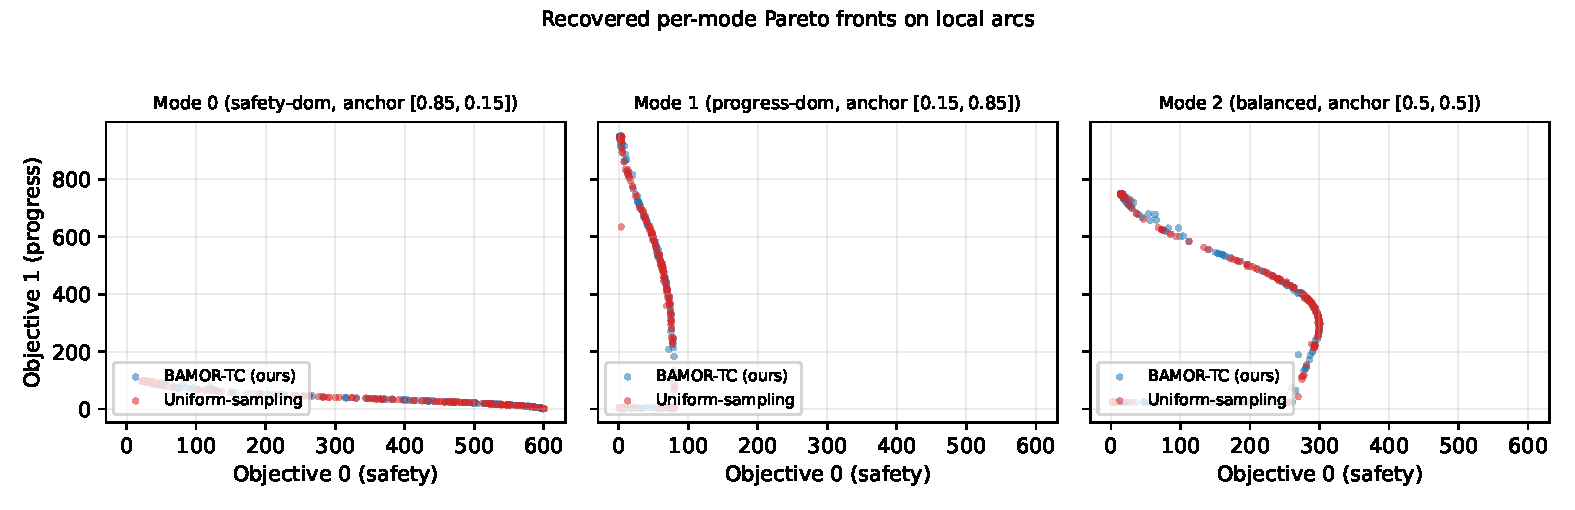
\includegraphics[width=0.98\linewidth]{fig_pareto_permode.pdf}
\caption{Per-mode Pareto fronts recovered by BAMOR-TC and Uniform, pooled across seeds and weights in the evaluation grid. Mode~0's front is a near-horizontal arc (progress capped), Mode~1's is near-vertical (safety capped), and Mode~2 is a full elbow. Both methods recover the same mode-wise geometry, while Uniform shows more low-return scatter in several panels.}
\label{fig:pareto_permode}
\end{figure}

Fig.~\ref{fig:pareto_permode} illustrates the different return geometries of the three synthetic modes. These are separate mode-conditioned fronts; their union is not the Pareto front of a single common evaluation task.  The substrate caps in Modes~0 and~1 appear as near-horizontal and near-vertical arcs respectively.  Uniform produces the same general shape but with more low-return/off-arc scatter in several panels.  BAMOR-TC's target-cone sampler targets each arc directly.

% ── 6.5 Training dynamics ───────────────────────────────────────────────────
\subsection{Training dynamics and stability}

\begin{figure}[t]
\centering
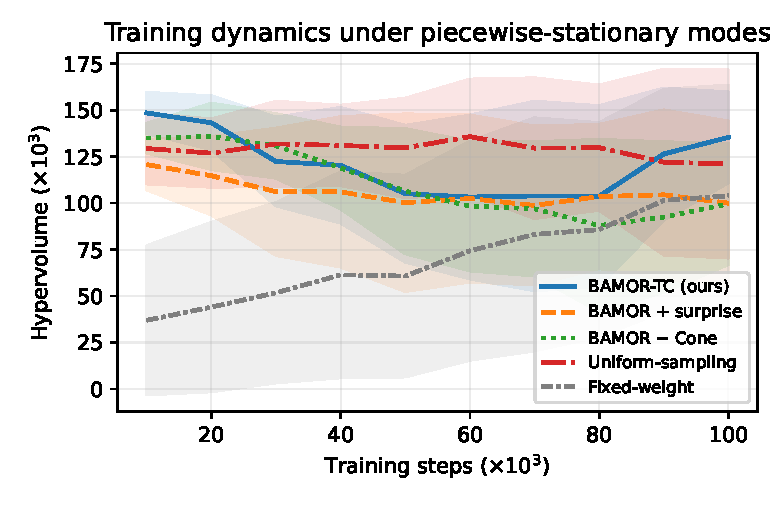
\includegraphics[width=0.72\linewidth]{fig_training_curves_v2.pdf}
\caption{Overall HV during training.  Shaded bands are $\pm1\sigma$ across 20 seeds.  BAMOR-TC (blue) starts high, loses ground in the middle training window, then recovers after $80$k steps and finishes with the highest mean and a tighter final band than Uniform.  Uniform (red) is steadier through the middle but ends lower.  BAMOR $+$ surprise (orange) and BAMOR $-$ Cone (green) finish well below BAMOR-TC.  Fixed-weight (grey) improves late but remains high-variance.}
\label{fig:training_curves}
\end{figure}

Fig.~\ref{fig:training_curves} shows HV trajectories during training.  Two qualitative patterns stand out.  First, BAMOR-TC is not a pointwise-dominant training curve: it starts high, falls below Uniform in the middle window, and then recovers sharply by the final evaluations.  The defensible claim is final HV and lower final variance, not monotone dominance at every checkpoint.  Second, both adaptive ablations have lower final sample means than BAMOR-TC. The paired synthetic comparison and ablation limitations above restrict a causal interpretation of these curves.

% ── 6.6 Continuous-control stress test ─────────────────────────────────────
